\chapter{Mediu virtual - Particularizare}

Pentru acest proiect am folosit una din versiunile dedicate dezvoltatorilor Oculus Riftu-ului și anume \textit{Developement kit 2}, în combinație cu dispozitivul \textit{Leap Motion} pentru crearea unui mediu virtual în care putem explora o galerie de artă, plasată într-o atmosferă futuristă.

\begin{figure}[h]
  \centering
  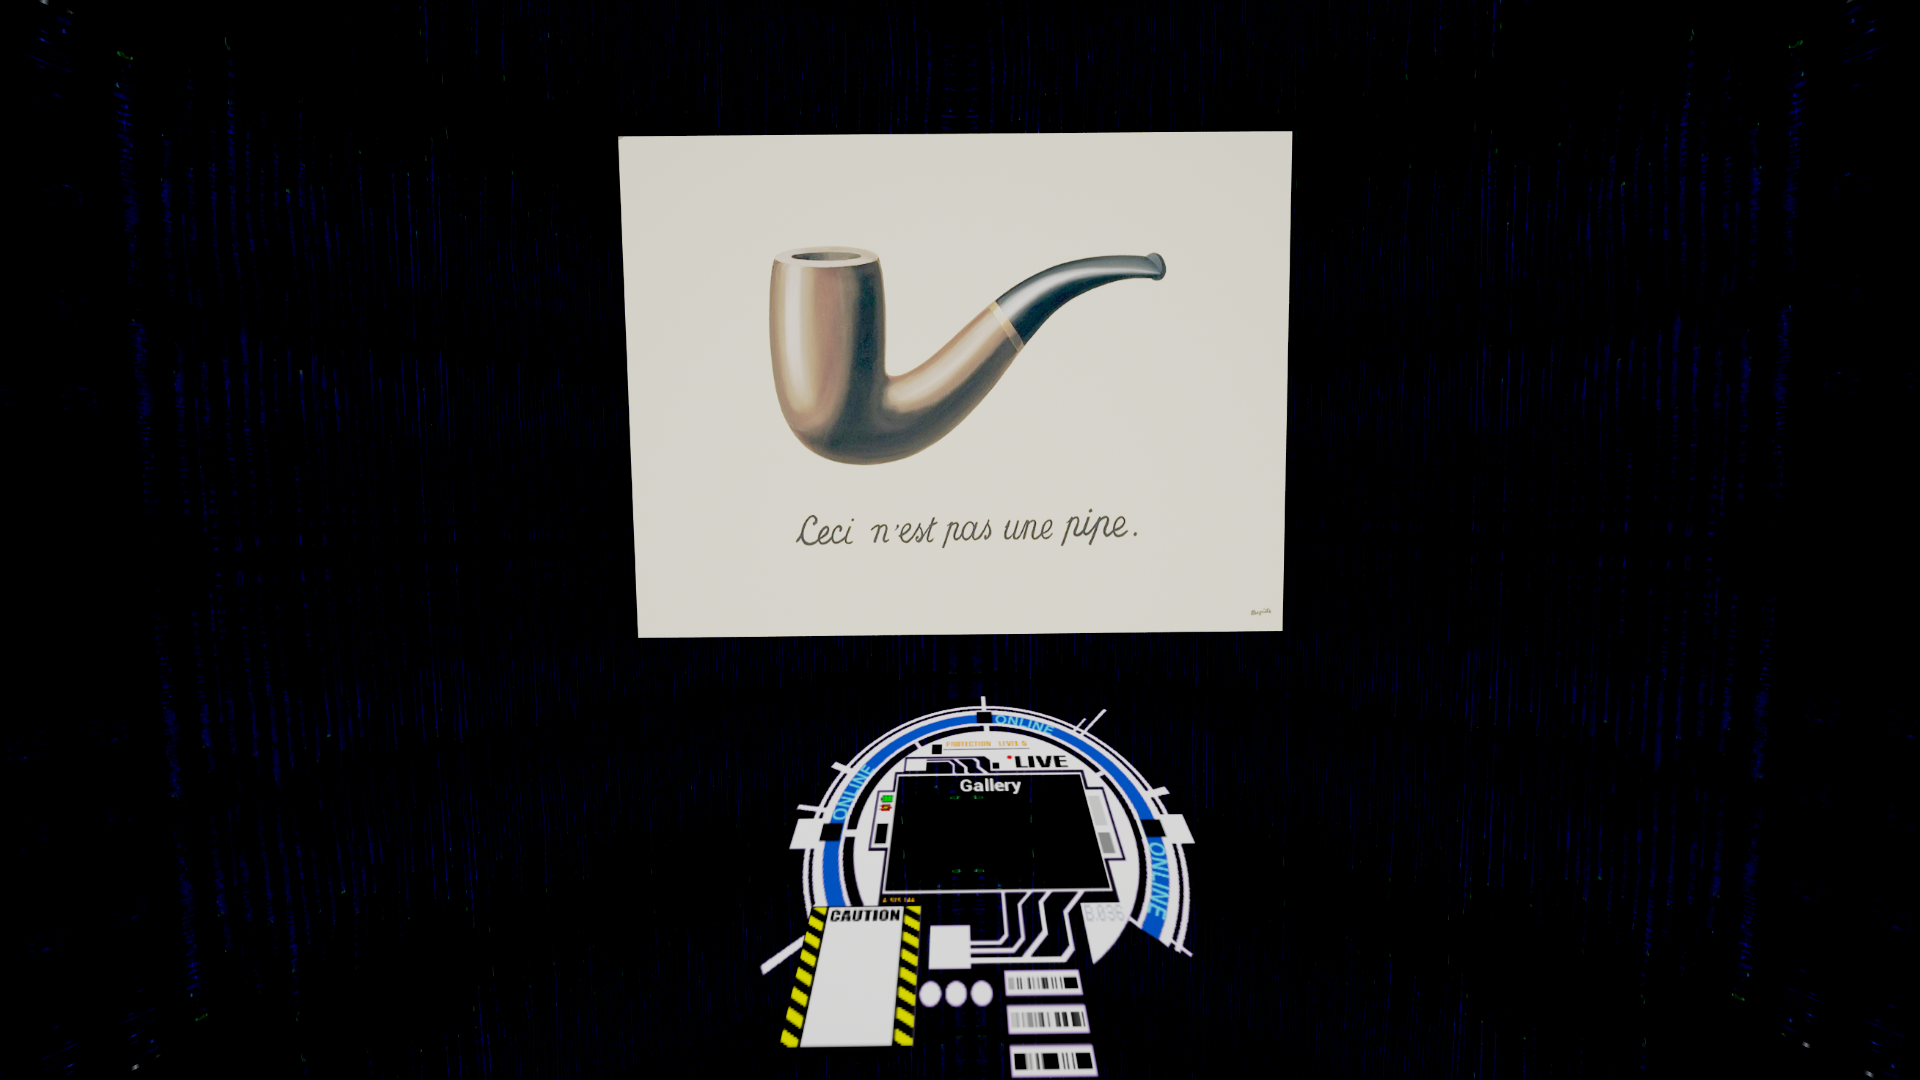
\includegraphics[scale=0.28]{img/screenshot2.png}
  \caption{Captură de ecran al aplicației 3D}
\end{figure}

Ceea ce scoate în evidență prezentarea și explorarea unor elemente într-un spațiu virtual comparativ cu utilizarea browserului într-un plan 2D, este libertatea creatorului de a-și exprima ideile și de a le plasa exact în atmosfera dorită, creând o proiecție a imaginației sale. Imersiunea utilizatorului nemaifiind obstrucționată de elemente externe, acesta fiind înconjurat doar de lucruri intenționat plasate.

Există experiențe ce pur și simplu nu pot fi redate prin medii clasice, vizitarea unui muzeu de artă spre exemplu. Deși imaginile picturilor pot fi găsite în cărți sau pe internet, grandoarea operelor este imposibil de capturat prin astfel de medii. Este o experiență complet diferită între a vedea o imagine de câțiva centimetri pe un monitor și de-a o avea în față la dimensiunile unui perete, într-un mediu liniștit fără a fi distras de elemente intruzive.


Un alt use case ce poate fi îndeplinit de această aplicație este de a păstra și explora un album foto, acesta putând fi structurat după preferință.
De asemenea în acest mediu pot fi redate și clipuri video,  putând servi ca un cinematograf personal.


Scopul acestei aplicații este de a demonstra un nou mod de interacțiune cu elemente virtuale, prin simpla folosire a mâinilor, un mod de a controla informația digitală folosindu-ne cele mai umane acțiuni.
De asemenea se exemplifică un mod de explorare a resurselor web în acest mediu, pentru a sublinia potențialul realității virtuale de a deveni un \textit{medium}.

În cazul nostru am folosit platforma XWiki pentru stocarea datelor pe baza cărora se generează principalele elemente grafice din interiorul aplicației.
Din punctul de vedere al utilizatorului aplicația poate fi descompusă în câteva elemente simple: spațiul în care este plasată\footnote{Decorul reprezintă o viziune personală a spațiului cibernetic, cu evidente influențe din \textit{Matrix} și \textit{Ghost in the Shell}.}, niște pseudo-panouri de control cu ajutorul cărora se pot alege și vizualiza operele artistice și proiecția picturii propriu-zise ce poate fi activată sau dezactivată din panoul principal.

Din punct de vedere tehnic, proiecția menționată anterior este un browser web virtual, setat să afișeze imaginile stocate în acest scop pe paginile wiki aferente, panoul principal este o reprezentare a paginii curente, iar cele secundare reprezintă copiii acesteia, afișând doar anumite informații extrase din paginile web.

\begin{figure}[h]
  \centering
  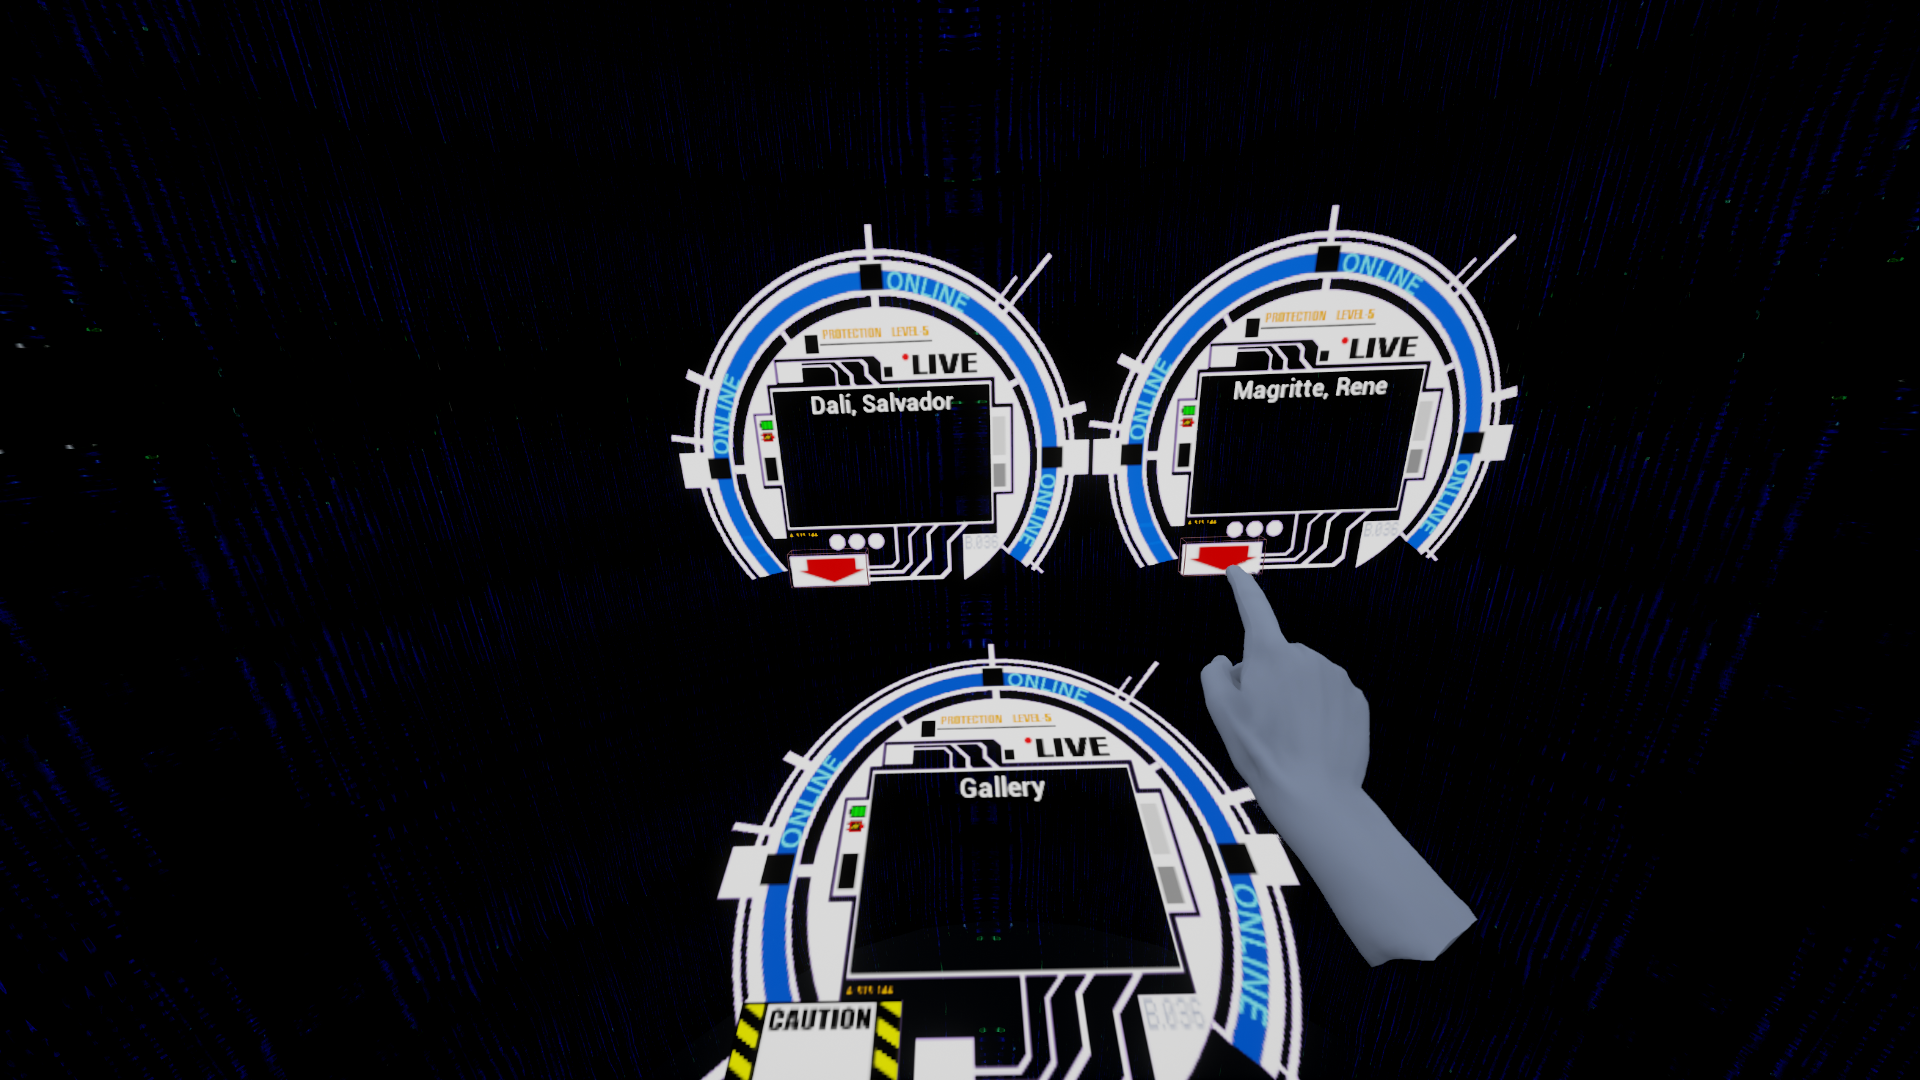
\includegraphics[scale=0.28]{img/screenshot1.png}
  \caption{Captură de ecran a aplicației 3D}
\end{figure}


\section{Implementare}

Pentru implementarea acestei aplicații am ales utilizarea motorului grafic \textit{Unreal Engine}, versiunea 4.12, datorită suportului pentru dispozitivele Oculus Rift și Leap Motion, și a comunității mari și active de utilizatori.

Pentru afișarea tridimensională pe ecranul căștii de realitate virtuală, și utilizarea senzorilor de mișcare ale acesteia am folosit plugin-urile \textit{Oculus Rift} și \textit{biblioteca Oculus}, oferite de Unreal Engine.

Realitatea virtuală păcălește creierul în a crede ca te afli într-o lume tridimensională, efect creat de un afișaj stereoscopic. Acest lucru funcționează afișând câte o imagine, pentru fiecare ochi, a aceleiași scene din două unghiuri ușor diferite, simulând distanța.

\begin{figure}[h]
  \centering
  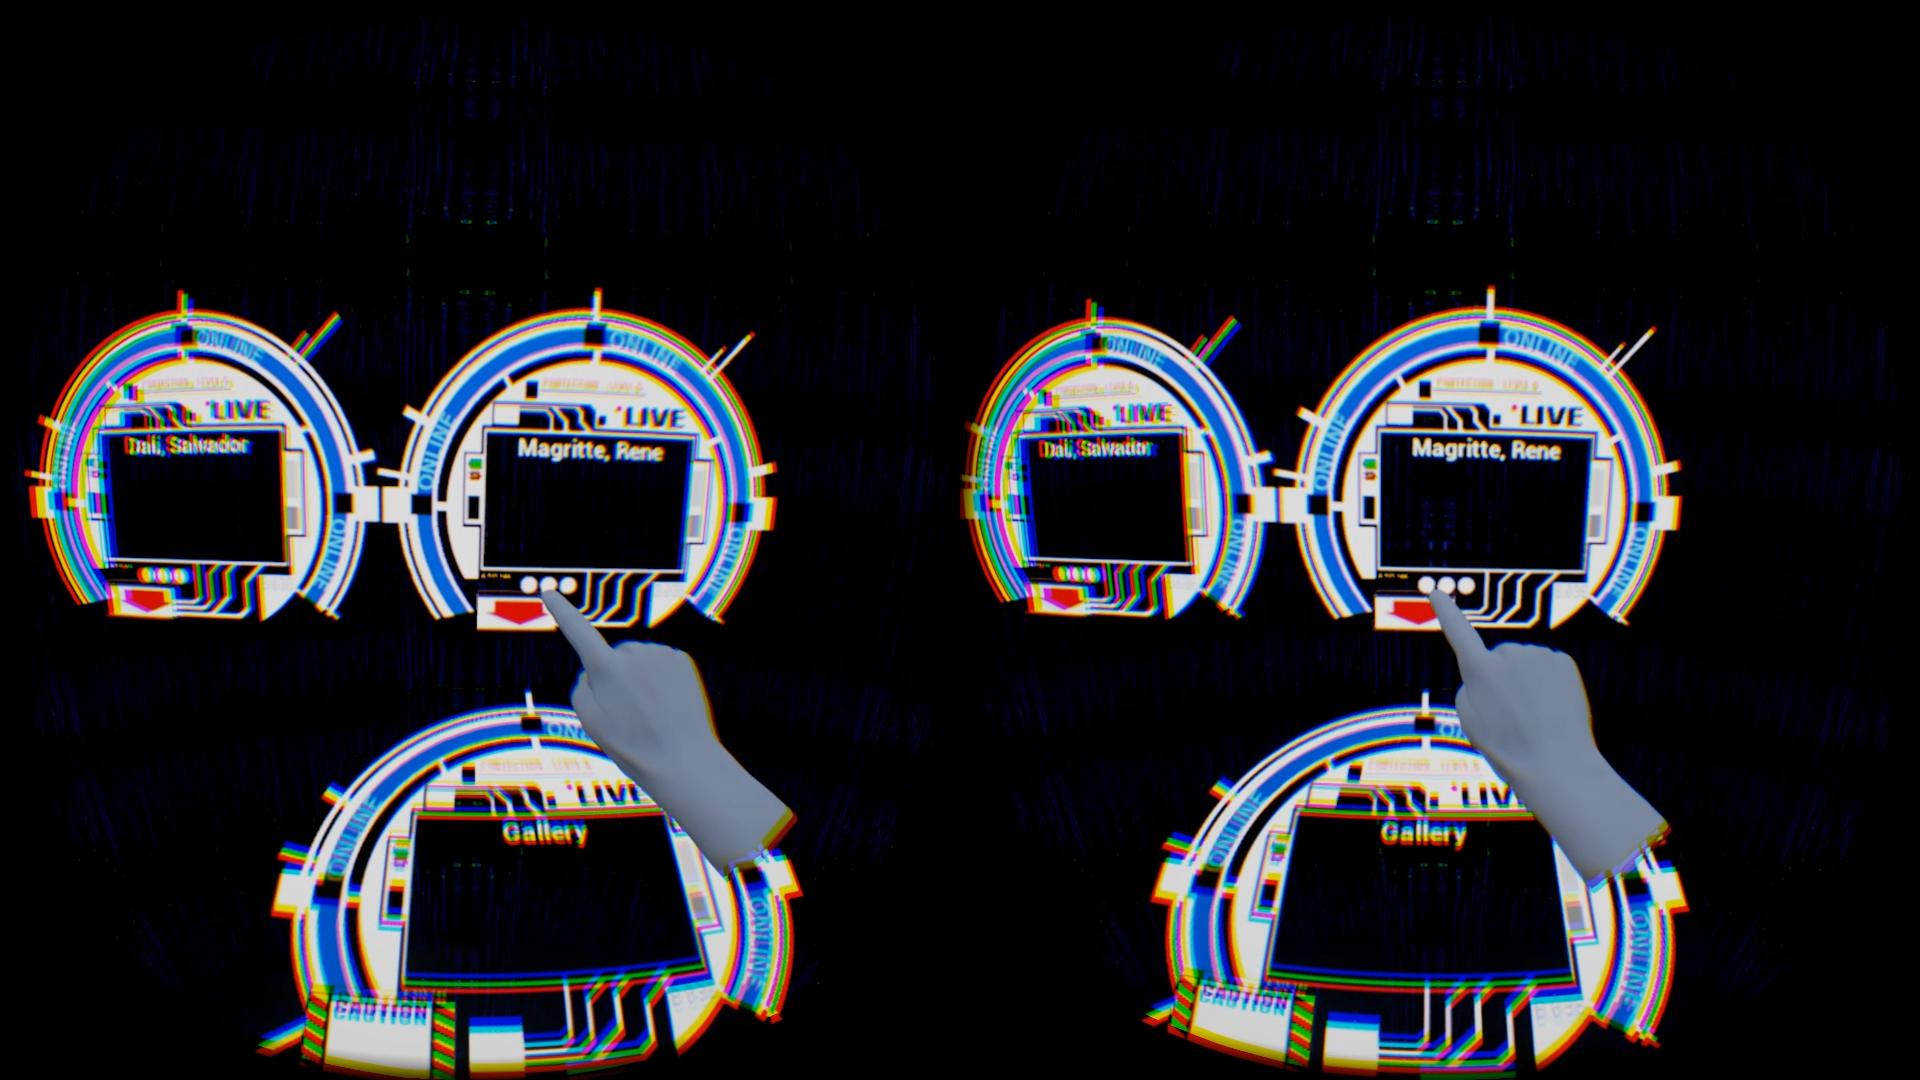
\includegraphics[scale=0.28]{img/stereoscopic.png}
  \caption{Afișaj stereoscopic ce crează efetul de distanță}
\end{figure}

Pentru captura și transpunerea mâinilor în spațiul virtual cum este observabil și în imaginea de mai sus, am utilizat plug-inul \textit{Leap Motion}, ce vine cu o varietate de opțiuni în ceea ce privește caracterul principal, ce funcționează împreună cu Oculus Rift, cum ar fi simularea unui corp a cărui mâini pot fi controlate cu Leap Motion, iar camera (punctul de vedere al jucătorului) va fi la nivelul ochilor acestui caracter, sau un caracter ce are doar mâinile prezente, în stilul jocurilor \textit{First-person shooter}. 
În cazul nostru am ales \textit{LeapFloatingHandsCharacter}, un caracter imaterial în care mâinile vor fi prezente doar în cazul detecției de către dispozitivul Leap Motion. Acest Plug-in ne oferă și posibilitatea de a face diferite acțiuni folosind gesturi ale mâinii ca metodă de input, spre exemplu pentru a putea vedea mai bine picturile, putem strânge pumnul stâng iar panourile vor dispărea. Repetarea mișcării le va aduce înapoi.


În ceea ce privește implementarea propriu-zisă, după cum am menționat anterior, Unreal Engine oferă atât posibilitatea utilizării unui limbaj vizual de scripting cât și programarea în limbajul C++.
Aici am folosit o combinație intre aceste moduri, sistemul de blueprint-uri pentru implementarea elementelor grafice și stabilirea interacțiunilor dintre ele, iar C++ pentru accesarea documentelor XWiki, parsarea XML-urilor returnate în urma apelurilor REST, și modificarea URL-urilor după caz.

\subsection{Blueprint-uri}

Am început prin a crea într-un spațiu gol, mediul ambiant ce este constituit dintr-o sferă goală, translucidă în centru căreia se află o platformă de sticla pe care stă personajul.
Sfera este la bază ceea ce în limbajul motoarelor grafice se numește un \textit{actor}\footnote{Un obiect ce poate fi plasat spațiul tridimensional, ce suportă transformări cum ar fi \textit{translație, scalare} sau \textit{rotație}} de tip \textit{static mesh}\footnote{Formă geometrică construită dintr-un set de poligoane ce este stocată în memoria video și randată de placa video}, asupra căreia am aplicat o serie de customizări pentru a crea efectul că suntem înconjurați de informații digitale în starea lor „naturală” în stilul filmului Matrix.

Acest efect a fost obținut prin crearea unui \textit{material}\footnote{Element ce poate fi aplicat unui \textit{mesh} pentru a-i schimba aspectul vizual} special format dintr-o imagine clasică, un negativ al imaginii (utilizat pentru obținerea transparenței) și un set de reguli pentru a dinamiza materialul.

\begin{figure}[h]
  \centering
  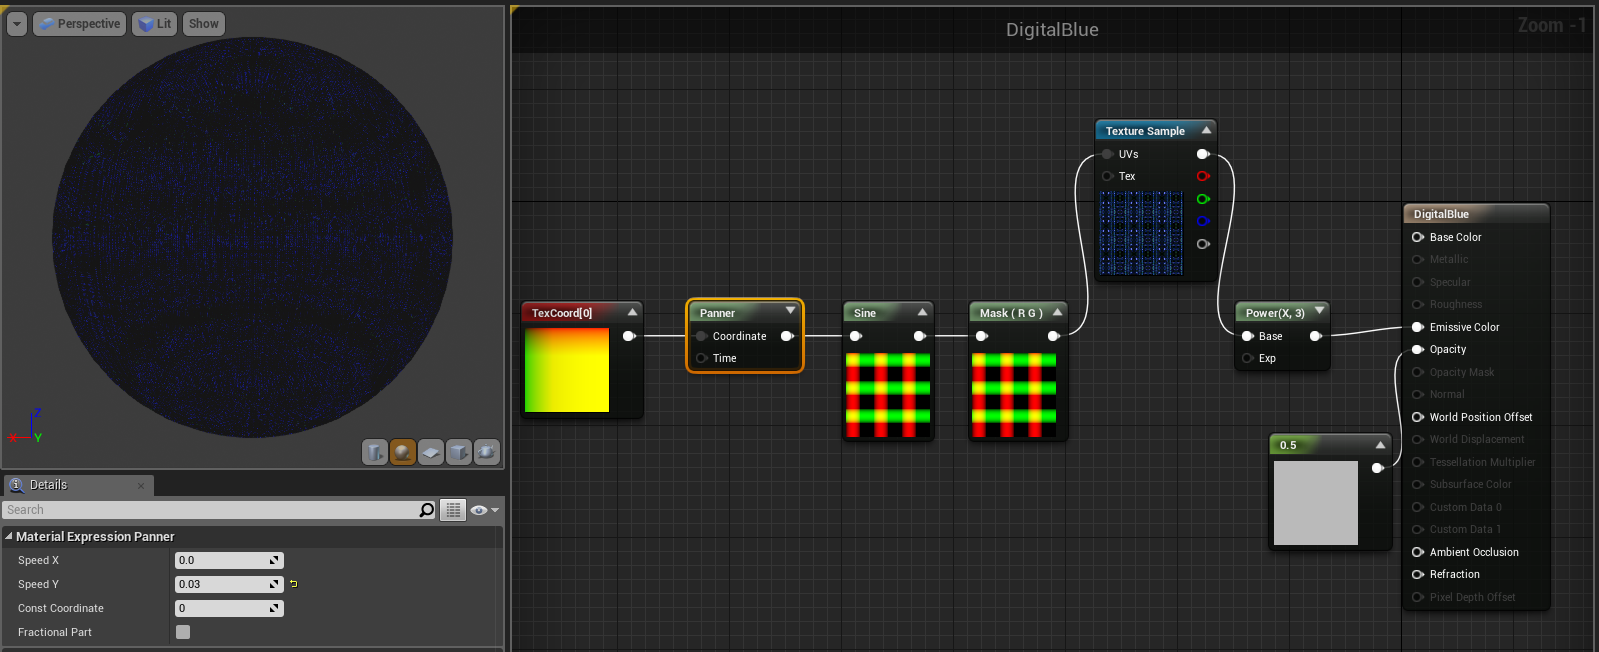
\includegraphics[scale=0.33]{img/digitalBlue.png}
  \caption{Blueprint ce conține regulile materialului dinamic aplicat sferei ambientale}
\end{figure}

Elementele interactive au fiecare asociate câte un \textit{actor} și un \textit{widget blueprint}.
Ecranul digital pe care afișăm imaginile este constituit dintr-un widget blueprint ce are la bază un \textit{canvas} în care este încărcat un browser web, și actorul ce are drept \textit{componentă}\footnote{Un tip special de obiect menit să fie utilizat ca sub-obiect în interiorul unui \textit{actor}. Sunt în general utilizate acolo unde este nevoie de părți modificabile.} widget-ul, căruia i se stabilesc niște setări de afișaj. Actorul primește ca parametru URL-ul imaginii pe care o va afișa browserul și implementează o funcție de schimbare a stării de vizibilitate a acestuia.
\newpage

\begin{figure}[h]
  \centering
  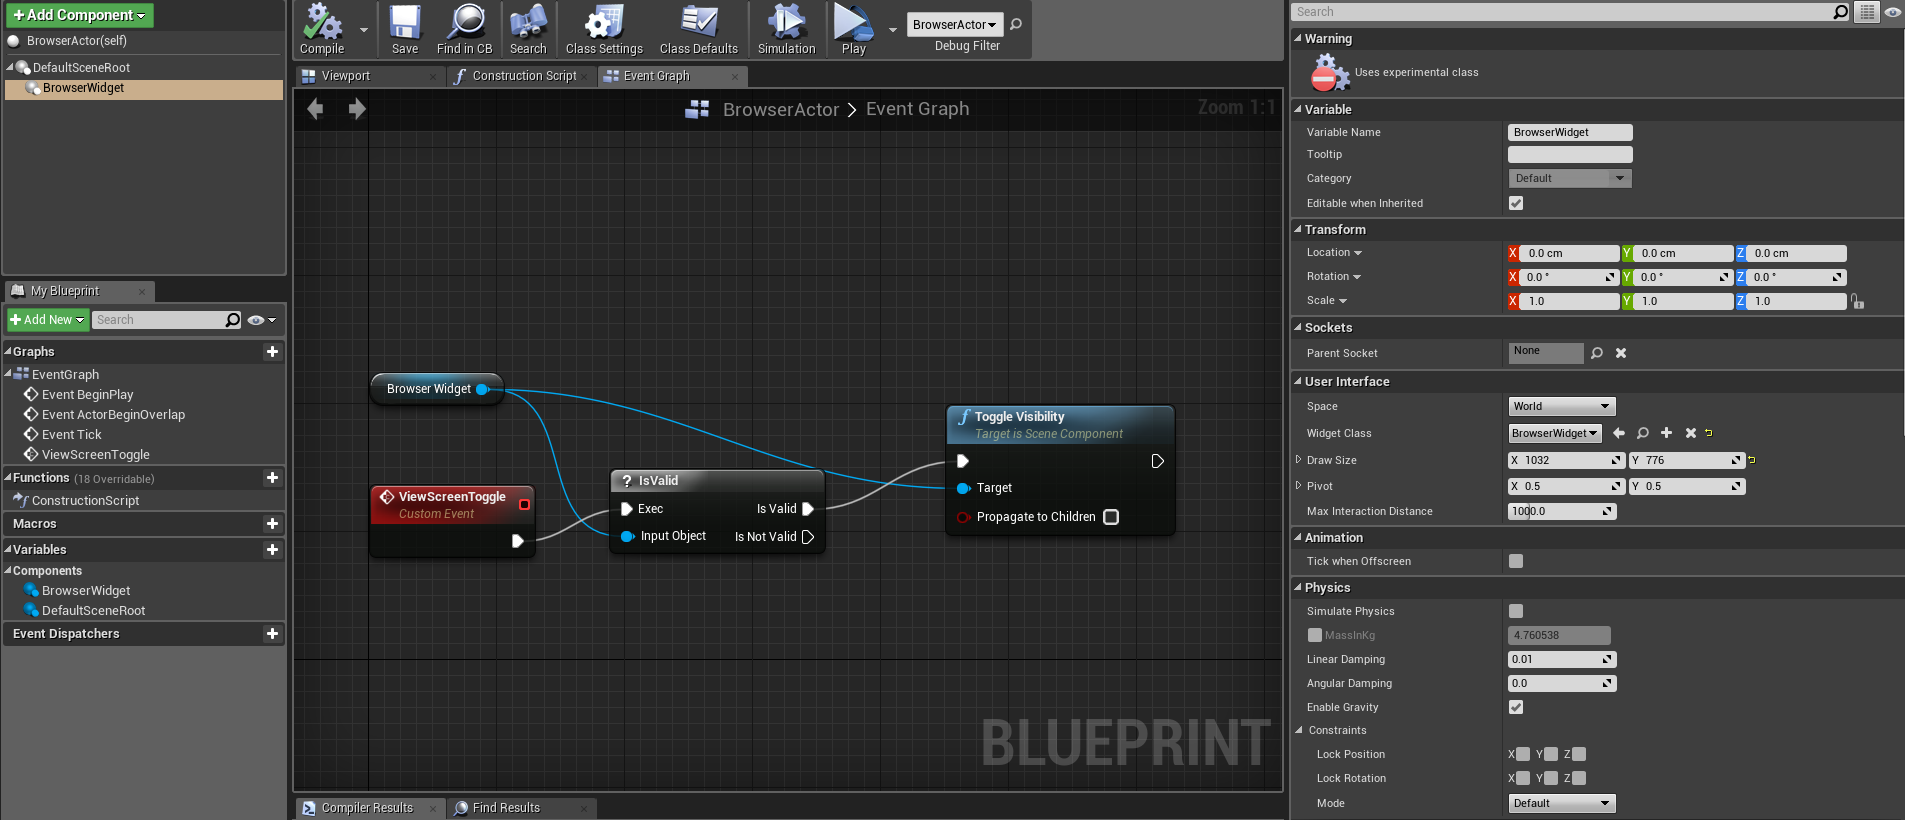
\includegraphics[scale=0.28]{img/toggleVisBrowserActor.png}
  \caption{Funcția de schimbare a stării de vizibilitate implementată de \textit{browser actor}}
\end{figure}
 
Panoul principal din fața utilizatorului este o instanță a unui actor ce conține mai multe componente: un \textit{widget} în care se găsesc o imagine și un bloc text, conținute de un canvas; \textit{LeaptController} componentă de care avem nevoie pentru a putea face referință la \textit{LeapRiggedEchoHeandsActor}, actorul ce reprezinta mâinile virtuale implementat de plug-in-ul \textit{Leap Motion}; și \textit{treeNodeComponent} ce este o clasă C++ în care procesăm paginile web și la care vom reveni ceva mai târziu.

Acest panel are două roluri importante, afișează informații despre pagina curentă și transmite către \textit{BrowserActor} (ecranul în care afișăm imaginile), URL-ul primei imagini din pagina curentă marcate ca fiind \textit{pictură} sau \textit{fotografie}.
Pentru a vedea cum sunt afișate și actualizate informațiile în blocul text al panelului trebuie șă analizăm următoarele scripturi implementate de actorul panelului.

\begin{figure}[h]
  \centering
  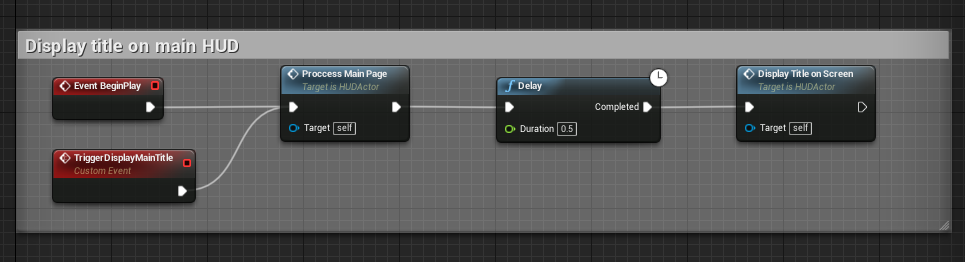
\includegraphics[scale=0.55]{img/DisplayTitleScript1.png}
  \caption{Scriptul principal de afișare a titlului în ecranul panelului}
\end{figure}

\textit{Event BeginPlay} este o funcție standard ce marchează începutul rulării programului, iar \textit{TriggerDisplayMainTitle} este un eveniment personalizat ce este apelat de utilizator când accesează o pagină copil. Ambele evenimente declanșează funcția \textit{ProccessMainPage}, ce apelează componenta C++ responsabilă cu procesarea paginii web și va actualiza lista cu informații selectate din aceasta, dupa care funcția \textit{DisplayTitleOnScreen} va seta valoarea textului afișat, în funcție de informația primită.
\newpage

\begin{figure}[h]
  \centering
  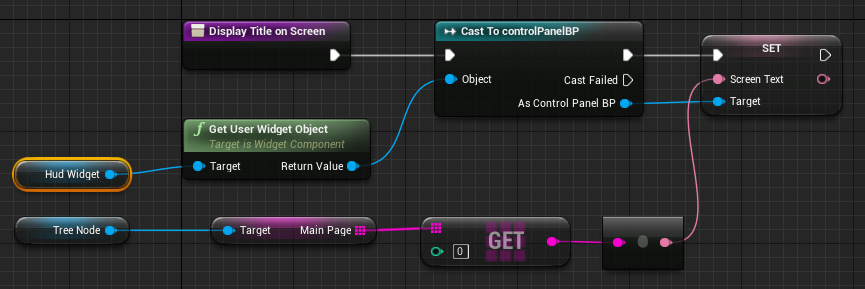
\includegraphics[scale=0.6]{img/DisplayTitleScript2.png}
  \caption{Conținutul funcției \textit{DisplayTitleOnScreen}}
\end{figure}

În figura 3.7 observăm conținutul funcției de afișare/actualizare a titlului paginii principale. Ramura de jos reprezintă lista cu informații despre pagina curentă returnată de componenta \textit{TreeNode} din care se selectează doar elementul cu indexul 0 ce întotdeauna va reprezenta titlul paginii. Acest element va deveni valoarea variabilei \textit{ScreenText} afișate de widget (\textit{controlPanelBP}).

Panourile secundare cu care utilizatorul poate interacționa pentru a selecta printre copii paginii curente au o construcție similară cu panoul principal cu excepția faptului că nu au un loc fix în spațiu. Ele sunt generate în fața utilizatorului pe baza informație primite în urma procesării paginii principale. Fiecare panou are asociate informații referitoare la pagina copil pe care o reprezintă, obținute prin folosirea API-ului REST oferit de platforma XWiki.

Actorul acestor panouri conține în principiu aceleași componente ca cel al panoului principal, \textit{TreeNode} pentru a avea acces la lista cu date despre pagina pe care o reprezintă, \textit{LeapController} pentru ca utilizatorul să le poată muta sau apăsa butoanele acestora, dar o diferență importantă este că acesta conține un container în care widget-urile vor fi generate ca sub-componente a acestuia în funcție de numărul copiilor paginii curente.
În urma selectării unuia dintre copii, URL-ul asociat acestuia va fi încărcat și procesat acesta devenind pagină principală iar lista componentelor va fi actualizată.


\begin{figure}[h]
  \centering
  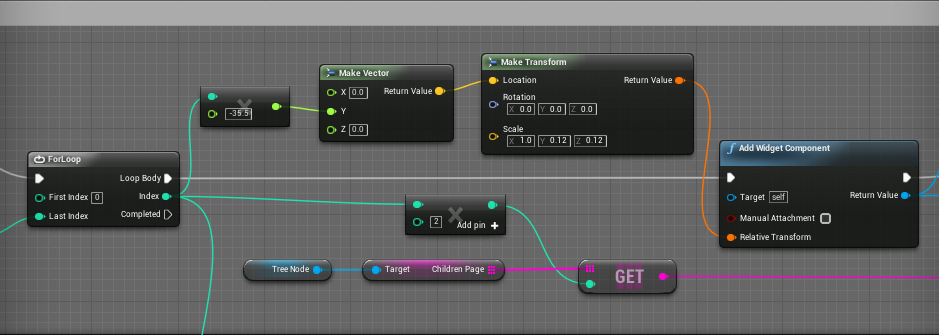
\includegraphics[scale=0.55]{img/SnipetTransform.png}
  \caption{Snippet din scriptul actorului \textit{ChildActor} responsabil cu calcularea pozițiilor în spațiu a panourilor generate}
\end{figure}

\subsection{C++}

În ceea ce privește programarea C++, se poate face din IDE-ul preferat, iar în acest caz am ales Visual Studios 2015 datorită suportului nativ și a funcției de \textit{hot reload}.
API-ul de gameplay și clasele framework-ului Unreal sunt accesibile atât sistemului vizual de scripting cât și din C++.

Aici am utilizat C++ pentru crearea componentei \textit{TreeNodeComponent} de care am vorbit în secțiunea anterioară ce are rolul de a accesa, selecta și aduce informații relevante din documentele XWiki.
Această componentă face disponibile câteva lucruri pe care le accesăm din blueprint-urile discutate mai sus.

\begin{lstlisting}[breaklines=true, postbreak=\mbox{\textcolor{red}{$\hookrightarrow$}\space}, caption=Snippet din fișierul header al componentei \textit{TreeNode} în care se observă funcții și variabile utilizate în blueprint-uri]
public:	
	FHttpModule* Http;

	/* The actual HTTP call */
	UFUNCTION()
		void accessWebsite(FString urltoaccess);
	UFUNCTION(BlueprintCallable, category="WebAccess")
		void proccessURL(FString crtUrl);

	//Create children url from main url
	FString ConstructChildrenUrl(FString crtUrl);

	/*Assign this function to call when the GET request processes sucessfully*/
	void OnResponseReceived(FHttpRequestPtr Request, FHttpResponsePtr Response, bool bWasSuccessful);

	// Sets default values for this component's properties
	UTreeNodeComponent();

	// Called when the game starts
	virtual void BeginPlay() override;
	
	// Called every frame
	virtual void TickComponent( float DeltaTime, ELevelTick TickType, FActorComponentTickFunction* ThisTickFunction ) override;

	UPROPERTY(Category = CustomElements, EditAnywhere, BlueprintReadWrite)
		FString crtChildrenUrl;

	UPROPERTY(Category = CustomElements, EditAnywhere, BlueprintReadWrite)
		TArray<FString> mainPage;

	UPROPERTY(Category = CustomElements, EditAnywhere, BlueprintReadWrite)
		TArray<FString> childrenPage;
\end{lstlisting}

\textit{crtChildrenUrl} este adresa la care găsim informații referitoare la copii paginii curente, iar \textit{mainPage} și \textit{childrenPage} sunt liste ce conțin informații precise ca titlul, conținutul, adresa pentru pagina principala respectiv copii acesteia.

Pentru accesarea paginilor web am folosit biblioteca \textit{Http.h} iar pentru procesarea xml-urilor returnate am folosit bibliotecile \textit{XmlParser} și \textit{FastXml}, toate oferite de framework-ul Unreal.

Funcția \textit{accessWebsite} efectuează apelul http efectiv al cărei răspuns este procesat ulterior iar informațiile relevante sunt extrase și adăugate în listele corespunzătoare.

\begin{lstlisting}[breaklines=true, postbreak=\mbox{\textcolor{red}{$\hookrightarrow$}\space}, caption=Funcția ce efectuează apelul http]
/*Http call*/
void UTreeNodeComponent::accessWebsite(FString urltoaccess)
{
	TSharedRef<IHttpRequest> Request = Http->CreateRequest();
	Request->OnProcessRequestComplete().BindUObject(this, &UTreeNodeComponent::OnResponseReceived);
	//This is the url on which to process the request
	Request->SetURL(urltoaccess);
	Request->SetVerb("GET");
	Request->SetHeader(TEXT("User-Agent"), "X-UnrealEngine-Agent");
	Request->SetHeader("Content-Type", TEXT("application/xml"));
	Request->ProcessRequest();
}
\end{lstlisting}

\begin{lstlisting}[breaklines=true, postbreak=\mbox{\textcolor{red}{$\hookrightarrow$}\space}, caption=Codul funcție principale ce este apelabilă din scripturile blueprint]
void UTreeNodeComponent::proccessURL(FString crtUrl) {
	mainPage.Empty();
	childrenPage.Empty();
	crtUrl = crtUrl + "?xpage=xml";
	crtChildrenUrl = ConstructChildrenUrl(crtUrl);
	accessWebsite(crtUrl);
	accessWebsite(ConstructChildrenUrl(crtUrl));
}
\end{lstlisting}

\begin{lstlisting}[breaklines=true, postbreak=\mbox{\textcolor{red}{$\hookrightarrow$}\space},caption={Funcția ce parsează xml-ul returnat de \textit{http request}, și adaugă informații în listele menționate anterior}]
/*Assigned function on successfull http call*/
void UTreeNodeComponent::OnResponseReceived(FHttpRequestPtr Request, FHttpResponsePtr Response, bool bWasSuccessful)
{
	if (bWasSuccessful) {
		if (Request->GetURL().EndsWith("xpage=xml"))
		{
			//Load xml for main pages
			const FString XWNodeString = Response->GetContentAsString();
			FXmlFile * File = new FXmlFile(XWNodeString, EConstructMethod::ConstructFromBuffer);
			FXmlNode* pRoot = File->GetRootNode();

			FXmlNode* titleNode = const_cast<FXmlNode*>(pRoot->FindChildNode("title"));
			FString pageTitle = titleNode->GetContent();
			FXmlNode* contentNode = const_cast<FXmlNode*>(pRoot->FindChildNode("content"));
			FString pageContent = contentNode->GetContent();
			mainPage.Add(pageTitle);
			mainPage.Add(pageContent);

			File->Clear();
		}
		else if (Request->GetURL().EndsWith("pages/WebHome/children")) {
			//Load xml for pages with children lists, these need adjustment to work
			const FString XWNodeString = Response->GetContentAsString().RightChop(55).Replace(TEXT(">"), TEXT(">\n"));
			FXmlFile * File = new FXmlFile(XWNodeString, EConstructMethod::ConstructFromBuffer);
			FXmlNode* pRoot = File->GetRootNode();
			int32 noOfChildren = pRoot->GetChildrenNodes().Num();
			for (int32 i = 0; i < noOfChildren; i++)
			{
				FString childTitle = pRoot->GetChildrenNodes()[i]->FindChildNode("title")->GetContent();
				FString childUrl = pRoot->GetChildrenNodes()[i]->FindChildNode("xwikiAbsoluteUrl")->GetContent();
				if (childTitle != "Preferences") {
					childrenPage.Add(childTitle);
					childrenPage.Add(childUrl);
				}
			}

			File->Clear();
		}
		else {
			GEngine->AddOnScreenDebugMessage(1, 2.0f, FColor::Green, "Curent url is not supported.");
		}
	}
	else {
		GEngine->AddOnScreenDebugMessage(1, 2.0f, FColor::Green, "It appeares that the xwiki instance has not been initiated!");
	}
}
\end{lstlisting}

\section{Platforma XWiki}

XWiki este un software wiki open source scris în Java ce pune accent pe extensibilitate. Include editare WYSIWYG\footnote{Acronim pentru „what you see is what you get”, ce se traduce aproximativ cu: „rezultatul [pe care îl obțineți] este chiar ceea ce se vede”}, import/export de documente, adnotări semantice și etichetare, și management avansat de permisiuni.
Fiind o aplicație wiki, XWiki permite stocarea de date structurate și executarea scripturilor la nivel de server din interfața wiki. Scripturi în limbaje ce includ Velocity, Groovy, Python, Ruby și PHP pot fi scrise direct în paginile wiki folosind macrouri wiki.


Am folosit această platformă pentru a crea o structură arborescentă de documente ce constituie galeria de artă în format 2D, din care mai apoi folosindu-ne de API-ul REST oferit de XWiki  putem extrage resursele de care avem nevoie pentru crearea elementelor 3D.

\begin{figure}[h]
  \centering
  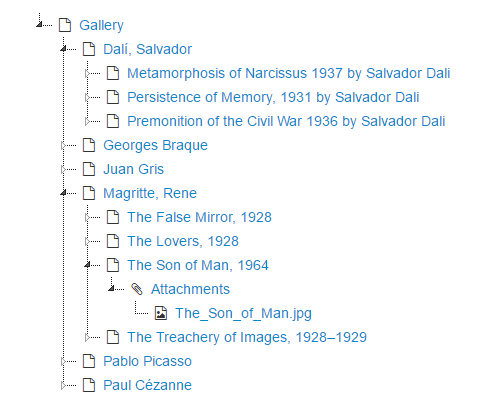
\includegraphics[scale=1.1]{img/docTree.png}
  \caption{Structura arborescentă a documentelor wiki}
\end{figure}
\clearpage

Pentru a putea parsa mai ușor conținutul unei pagini wiki am recurs la accesarea acestei în format xml, lucru posibil prin simpla apelare a acesteia cu parametrul \textit{xpage=xml}.
Acest lucru facilitează aplicației noastre izolarea și extragerea resurselor relevante cu ajutorul parserului xml.

\begin{figure}[h]
  \centering
  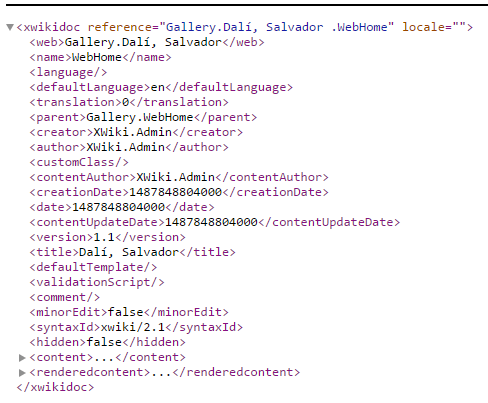
\includegraphics[scale=1.2]{img/xpagexml.png}
  \caption{Document wiki în format xml}
\end{figure}
\clearpage

URI-ul rădăcină a serviciului XWiki RESTful API este setat implicit la:

\textit{http://host:port/xwiki/rest}

Spre exemplu resursa \textit{/wikis} de pe un server ce rulează local pe portul 8080 poate fi accesată folosind următorul URL:

\textit{http://localhost:8080/xwiki/rest/wikis}

În cazul nostru am folosit acest serviciu pentru a determina copiii unei pagini. Conform documentației, URL-ul pentru a accesa acest tip de resursă va avea următoare formă:

\textit{/wikis/{wikiName}/spaces/{spaceName}[/spaces/{nestedSpaceName}]*/pages/{pageName}/children}

\begin{figure}[h]
  \centering
  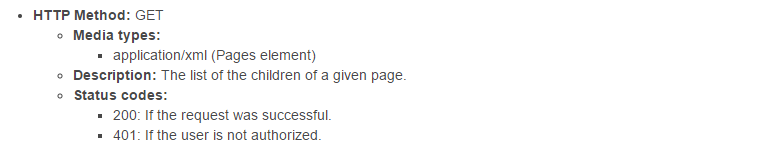
\includegraphics[scale=1]{img/restAPI.png}
\end{figure}

\section{Funcționalități de adăugat}

Deși dispozitivul Leap Motion este impresionant în abilitatea lui de a captura și transpune mâinile în obiecte virtuale, tehnologia este abia la început iar în practică, acuratețea acestui lasă de dorit. Din acest motiv, adăugarea suportului pentru metode de input mai precise, cum ar fi controlerele Vive sau Oculus Touch, va fi pe lista lucrurilor de adăugat în viitor.

O altă funcționalitate ce ar oferi un plus de valoare aplicației ar fi adăugarea posibilității mai multor persoane de a se conecta, întâlni și comunica în cadrul aceleași instanțe, lucru ce ar extinde considerabil aria de use case-uri.